\section{Resultados}\label{sec:resultados}

\begin{table}[h!]
    \footnotesize
    \caption{Tabla de datos. Intensidad de la corriente $I$ y diferencia de potencial $\Delta V$, para diferentes longitudes $L$
        y secciones $S$.}
    \label{tab:1-t4-20}
    \begin{centering}
        \begin{tabular}{|P{17px}|P{22px}|P{31px}|P{22px}|P{31px}|P{22px}|P{31px}|}
            \hline
            \multicolumn{1}{|c}{} & \multicolumn{2}{|c}{$S = 1.5\,$mm$^2$} & \multicolumn{2}{|c}{$S = 0.5\,$mm$^2$} & \multicolumn{2}{|c|}{$S = 0.32\,$mm$^2$} \\
%            $L$       & $I$       & $\Delta V$       & $I$       & $\Delta V$       & $I$       & $\Delta V$                             \\
            \hline
            $L\,$(m)       & $I\,$(mA) & $\Delta V\,$(mV) & $I\,$(mA) & $\Delta V\,$(mV) & $I\,$(mA) & $\Delta V\,$(mV) \\
            \hline
            \multirow{1}   & 50        & 1,4              & 50        & 2,3              & 50        & 2,9              \\
            & 100       & 2,5              & 100       & 4,7              & 100       & 6,1              \\
            & 150       & 3,8              & 150       & 7,2              & 150       & 9,2              \\
            & 200       & 5,2              & 200       & 9,7              & 200       & 12,6             \\
            & 250       & 6,8              & 250       & 12,1             & 250       & 15,7             \\
            & 300       & 8,0              & 300       & 14,5             & 300       & 18,6             \\
            \hline
            \multirow{1.5} & 50        & 1,6              & 50        & 5,6              & 50        & 5,3              \\
            & 100       & 3,5              & 100       & 11,3             & 100       & 11,1             \\
            & 150       & 5,1              & 150       & 17,1             & 150       & 19,3             \\
            & 200       & 6,7              & 200       & 22,5             & 200       & 23,2             \\
            & 250       & 8,6              & 250       & 28,0             & 250       & 29,6             \\
            & 300       & 10,3             & 300       & 33,4             & 300       & 35,4             \\
            \hline
            \multirow{2}   & 50        & 1,7              & 50        & 6,9              & 50        & 6,2              \\
            & 100       & 3,5              & 100       & 13,4             & 100       & 12,4             \\
            & 150       & 5,3              & 150       & 20,1             & 150       & 19,0             \\
            & 200       & 7,2              & 200       & 27,4             & 200       & 25,2             \\
            & 250       & 9,0              & 250       & 33,7             & 250       & 31,2             \\
            & 300       & 10,9             & 300       & 40,1             & 300       & 38,3             \\
            \hline
        \end{tabular}
    \end{centering}
\end{table}


\begin{figure}[h!]
    \begin{center}
        \includegraphics[width=0.8\columnwidth]{files/images/S1L1}
    \end{center}
    \caption{$\Delta V$ frente a $I$, cable $S = 1.5\,$mm$^2$ y $L = 1\,$m.}
    \label{fig:S1L1}
\end{figure}

\begin{figure}[h!]
    \begin{center}
        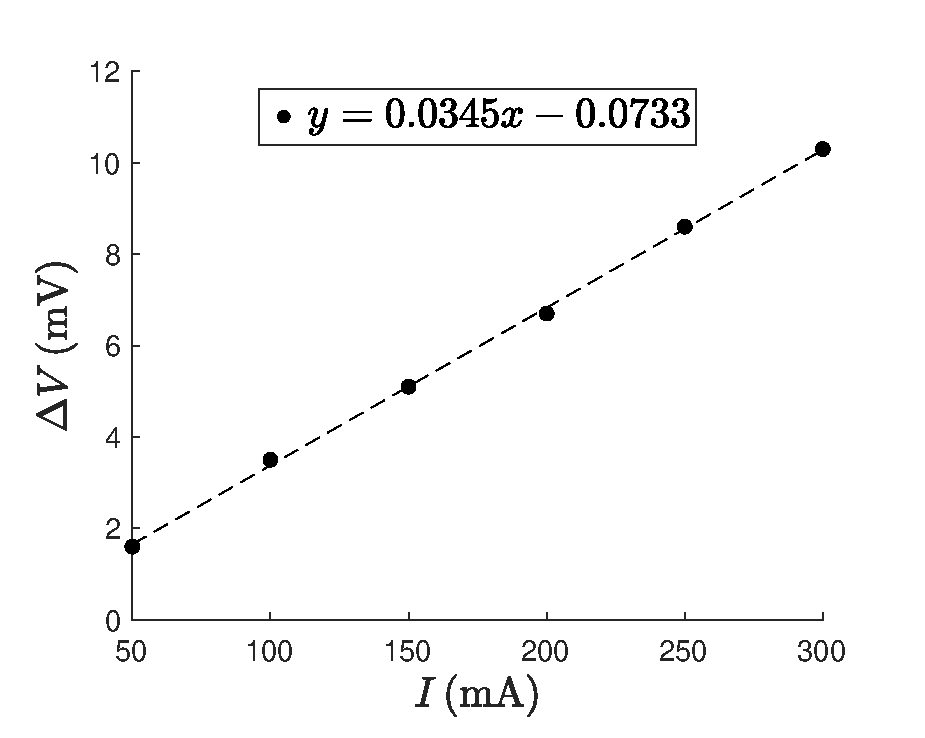
\includegraphics[width=0.8\columnwidth]{files/images/S1L2}
    \end{center}
    \caption{$\Delta V$ frente a $I$, cable $S = 1.5\,$mm$^2$ y $L = 1.5\,$m.}
    \label{fig:S1L2}
\end{figure}

\begin{figure}[h!]
    \begin{center}
        \includegraphics[width=0.8\columnwidth]{files/images/S1L3}
    \end{center}
    \caption{$\Delta V$ frente a $I$, cable $S = 1.5\,$mm$^2$ y $L = 2\,$m.}
    \label{fig:S1L3}
\end{figure}

\begin{figure}[h!]
    \begin{center}
        \includegraphics[width=0.8\columnwidth]{files/images/S2L1}
    \end{center}
    \caption{$\Delta V$ frente a $I$, cable $S = 0.5\,$mm$^2$ y $L = 1\,$m.}
    \label{fig:S2L1}
\end{figure}

\begin{figure}[h!]
    \begin{center}
        \includegraphics[width=0.8\columnwidth]{files/images/S2L2}
    \end{center}
    \caption{$\Delta V$ frente a $I$, cable $S = 0.5\,$mm$^2$ y $L = 1.5\,$m.}
    \label{fig:S2L2}
\end{figure}

\begin{figure}[h!]
    \begin{center}
        \includegraphics[width=0.8\columnwidth]{files/images/S2L3}
    \end{center}
    \caption{$\Delta V$ frente a $I$, cable $S = 0.5\,$mm$^2$ y $L = 2\,$m.}
    \label{fig:S2L3}
\end{figure}

\begin{figure}[h!]
    \begin{center}
        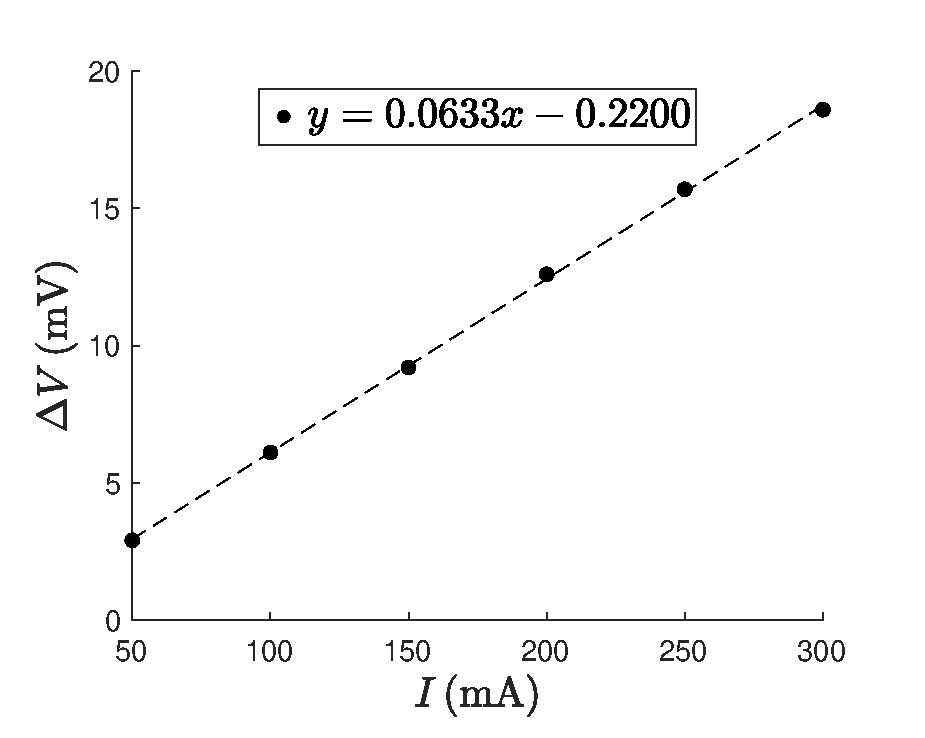
\includegraphics[width=0.8\columnwidth]{files/images/S3L1}
    \end{center}
    \caption{$\Delta V$ frente a $I$, cable $S = 0.325\,$mm$^2$ y $L = 1\,$m.}
    \label{fig:S3L1}
\end{figure}

\begin{figure}[h!]
    \begin{center}
        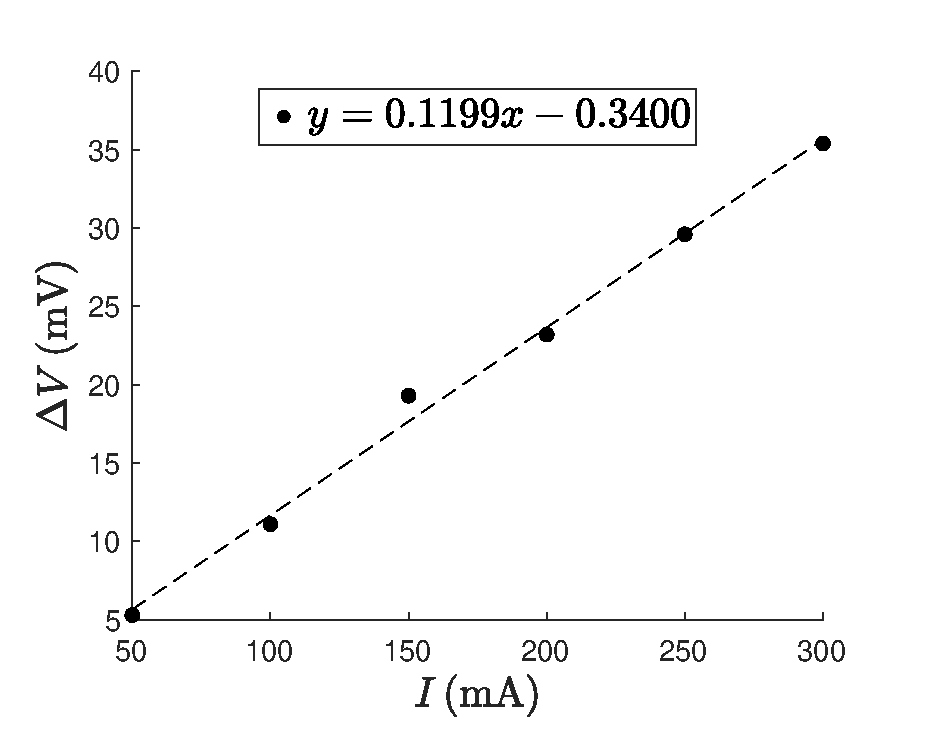
\includegraphics[width=0.8\columnwidth]{files/images/S3L2}
    \end{center}
    \caption{$\Delta V$ frente a $I$, cable $S = 0.32\,$mm$^2$ y $L = 1.5\,$m.}
    \label{fig:S3L2}
\end{figure}

\begin{figure}[h!]
    \begin{center}
        \includegraphics[width=0.8\columnwidth]{files/images/S3L3}
    \end{center}
    \caption{$\Delta V$ frente a $I$, cable $S = 0.32\,$mm$^2$ y $L = 2\,$m.}
    \label{fig:S3L3}
\end{figure}

